\documentclass[conference]{IEEEtran}

\usepackage{IEEEpreamble}
\usepackage{booktabs}

%\newcommand{\purpose}[1]{\textsc{\textbf{#1}}}
\newcommand{\purpose}[1]{}

\begin{document}
%
% paper title
% can use linebreaks \\ within to get better formatting as desired

\title{Commit Bubbles}

%\title{Flossy History Revision Editing for Version Control Commits}

% \title{Version control interventions: helping developers avoid cognitive breakdowns for more effective change management}

\author{\IEEEauthorblockN{Titus Barik,
Kevin Lubick,
Emerson Murphy-Hill}
\IEEEauthorblockA{North Carolina State University, USA\\
\{tbarik,kjlubick\}@ncsu.edu, emerson@csc.ncsu.edu}
}

% use for special paper notices
%\IEEEspecialpapernotice{(Invited Paper)}

% make the title area
\maketitle

\begin{abstract}
%\boldmath
When working with version control systems, developers are expected to produce systematic commit histories that show well-defined steps with logical forward progress. 
Existing version control tools assume that developers also write code systematically
and they can flawlessly
produce commit histories that satisfy these expectations.
In such a case, history revision would be rare. Yet, the process by which developers write source code is often evolutionary, or as-needed, rather than systematic.  Consequently, histories are rarely systematic without significant revision. Our insight is that by treating revision as a frequent and routine activity, developers can continue to work in their as-needed way, while simultaneously producing systematic histories. 
Our contribution is a fragment-oriented concept called Commit Bubbles that will allow developers to construct commit histories that adhere to version control best practices with less cognitive effort, and in a way that integrates with their as-needed coding workflows.
\end{abstract}

% no keywords

% For peer review papers, you can put extra information on the cover
% page as needed:
% \ifCLASSOPTIONpeerreview
% \begin{center} \bfseries EDICS Category: 3-BBND \end{center}
% \fi
%
% For peerreview papers, this IEEEtran command inserts a page break and
% creates the second title. It will be ignored for other modes.
\IEEEpeerreviewmaketitle

\begin{figure*}
\centering
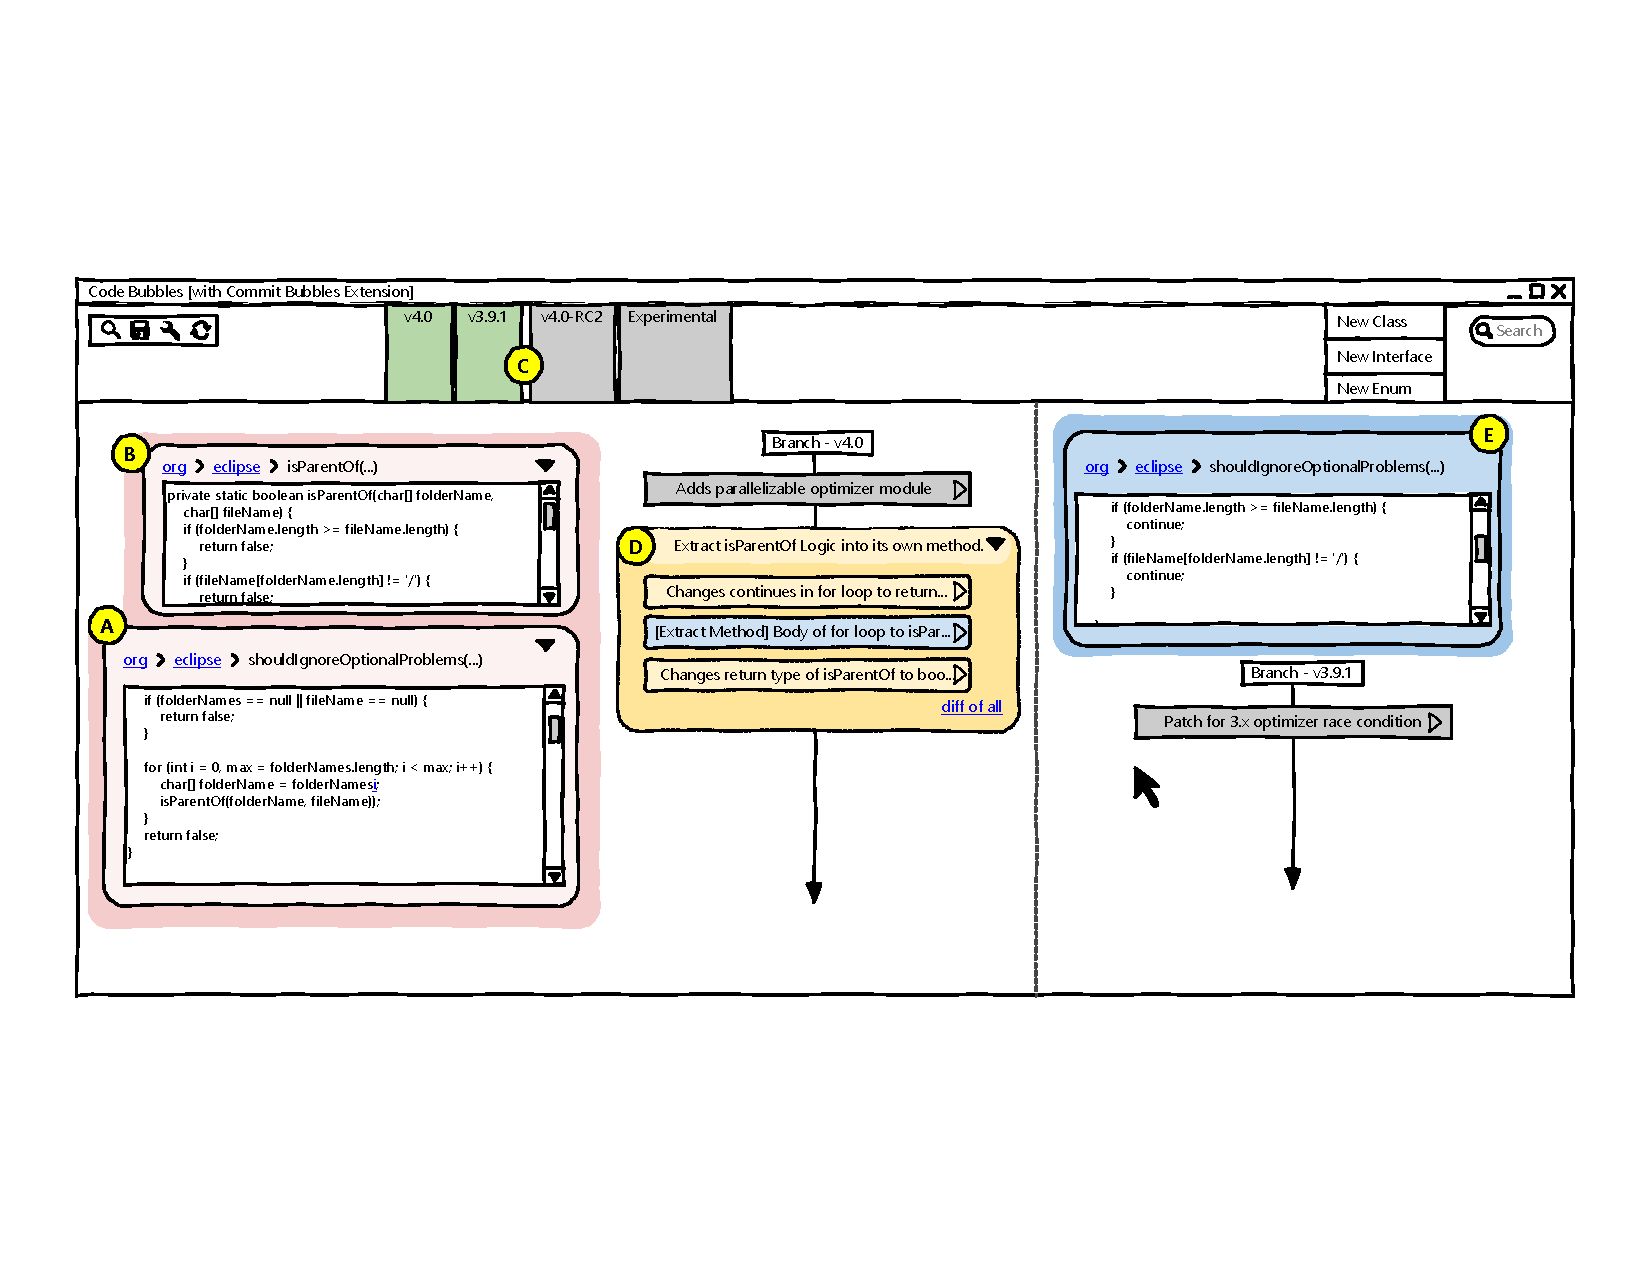
\includegraphics[width=\linewidth]{codebubbles}
\caption{A mockup of Code Bubbles, extended with Commit Bubble elements. 
(A), (B) and (D) are code bubbles, which can be placed on the screen by using the search bar (E) or a dragging-and-dropping from a navigation tree (not shown). 
(F) shows a task context, that is, a panel of working sets.
A commit bubble can be expanded (C) to reveal additional information. 
In this figure, (C) consists of two squashed commits, with a third commit bubble being added to this set using drag-and-drop. 
The environment offers an infinitely scrollable canvas where the developer performs both coding and commit activities.}
\label{fig:eclipse}
\end{figure*}

\section{Motivation}

\purpose{Best practices for version control commit messages.} 
In version control systems, a \emph{commit} represents an atomic set of changes with respect to a previous state; together, these sequences of commits form a \emph{commit history}~\cite{Loeliger2012}.
There are many best practices when adding commits to version control commit histories. 
For the commit itself, these best practices include using a descriptive commit message; 
avoiding \emph{indiscriminate} commits, that is, commits that blindly include all changed files; and making each commit a ``logical unit'' --- such that 
each commit has a singular purpose~\cite{GitBestPractices}.
Extending this idea, the resulting \emph{published} commit histories should, in some sense, be \emph{systematic}, 
in that the history shows well-defined steps, each with logical forward progress, telling a cohesive narrative without 
broken or suboptimal steps~\cite{Loeliger2012}.

\purpose{Coding activities use a different model than what VCS requires.} 
Yet the way in which developers write and edit source code is not commonly done in a \emph{systematic} way, but an \emph{as-needed} way instead~\cite{Perry1989,Littman1987}. 
When using a systematic strategy, developers first construct a plan to complete a set of tasks and only then make the edits (e.g. waterfall).
In contrast, when adopting an as-needed strategy, developers identify a relevant point in the program and continue making edits until the solution emerges (e.g. agile).
% Furthermore, Littman notes the dichotomy between systematic version histories and as-needed coding processes:
%  ``trying to force this evolutionary [coding] process into neat, distinct, and independent phases [commits] only serves
%   to obscure the reality of software development.''~\cite{Littman1987}

\purpose{Problem is that strategies are incompatible.} 
The fundamental problem is the as-needed strategy developers frequently use to write code is incompatible with 
the systematic strategy that developers would need to use in order to generate their published commit histories. 
As evidence, Murphy-Hill and colleagues found that refactoring operations are performed frequently, and that programmers 
frequently interleave refactoring with other types of programming activity~\cite{Murphy-Hill2012c}. 
Similarly, Negara and colleagues found that 46\% of refactored program entities are interspersed with other changes, and that 40\% of test fixes involve changes to the tests themselves~\cite{Negara2012}. 
In version control histories, these as-needed edits manifest themselves as \emph{tangled} commits, that is, commits that contain two or more logical units of changes~\cite{Kirinuki2014}, and as incomplete or incorrect commit messages, which fail to capture the full description of the change~\cite{Buse2010,Murphy-Hill2012c}. 
Both of these issues are obstacles to supporting downstream change management tasks, such as merging commits between branches, and conducting effective code reviews~\cite{Kirinuki2014}.

\purpose{History revision gets out of this conflict} 
A potential solution is to untangle commit histories into systematic histories using history revision operations offered by version control systems\footnote{Robertson calls this ``sausage making'' -- ``The process of developing software, 
similar to the process of making sausage, is a messy messy business $[\ldots]$ If you hide the sausage making, 
you can create a beautiful looking history where each step looks as delicious as the end-product.'' 
\cite{SausageMaking}}.
For example, a developer can theoretically reorder or delete commits using \textit{rebase}.
However, in practice, this procedure is difficult to perform correctly~\cite{SausageMaking}.

\purpose{History revisions are not properly supported by tools} 
In this paper, we argue that the primary barrier to performing effective history revision is that current revision tools inadequately align their tool 
functionality with developer workflows~\cite{PerezDeRosso2013}.
First, revision activities, if they occur at all, are typically performed as a distinct activity from coding~\cite{Perry1989}. 
This context switch makes it difficult to remember all of the change activities related to a particular commit, 
since human memory is particularly failure-prone during these switches~\cite{Parnin2012}. 
Second, history revision as supported in tools today takes the perspective that 
developers are ordinarily able to successfully create systematic histories, and that revision is an exceptional situation. However, research indicates that exceptions are normal in work processes, and tools should support handling 
exceptional situations as routine~\cite{Ackerman2000}.

\purpose{we envision a tool that treats history revision as routine and integrates it with coding} 
Our vision is a development model that reconciles as-needed coding activities with systematic commit activities.
We operationalize this model by adding commit support to \emph{Code Bubbles}, a metaphor and tool that allows developers
to reason in terms of fragments and working sets, and allows for fluid rearrangement and manipulation of these working sets~\cite{Bragdon2010a}.
%We postulate that developers can benefit from reasoning about commit activities in the same way. 
Our proposed extension, \emph{Commit Bubbles}, supports developers by a) blending coding and commit activities through fragments to  
minimize context switching, and b) treating history revision as a routine, rather than exceptional process. 
Our contribution is a concept that will allow developers to construct commit histories that adhere to version control best practices with less cognitive effort, and in a way that integrates with their as-needed coding workflows.

%\section{TACO -- Tool Assisted Commit Operations}
%\begin{figure}
%\centering
%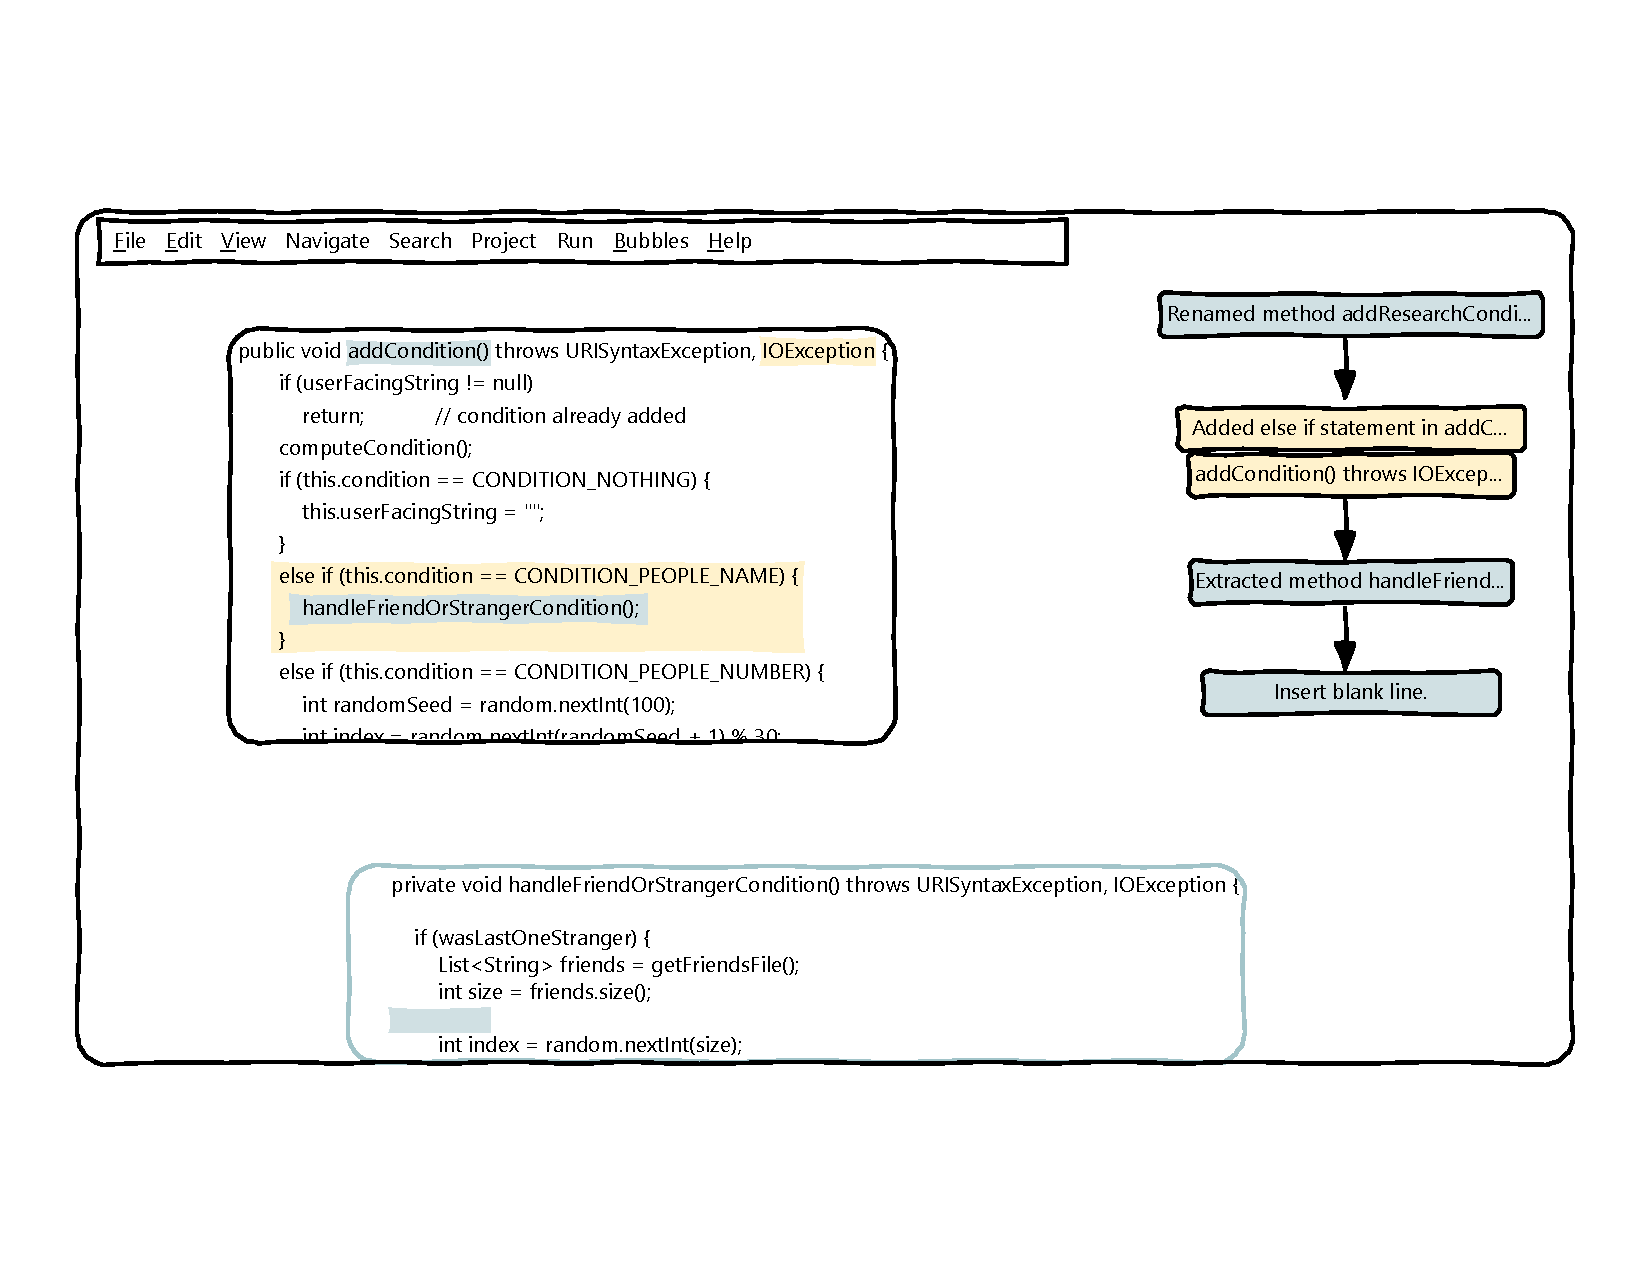
\includegraphics[width=3.5in]{commit-bubbles}
%\caption{A mockup of TACO, showing the commit bubbles (A), the mouseovers (B),
%and the change notifications (C)}
%\label{fig:eclipse}
%\end{figure}




\section{Commit Bubbles}

% exploratory programming

Researchers recognize the cognitive benefits of tools that support thinking in fragments, rather than files~\cite{Bragdon2010a,DeLine2010a,Henley2014,Coblenz2006}.
Fragments offer a metaphor for displaying relevant pieces of information in an as-needed way, for example, when coding or debugging. 
We postulate that version control activities frequently require fragment-based thinking, for example, when comparing code at two different states, when determining an atomic set of changes to commit, and when reordering commit histories.

We chose Code Bubbles to prototype our concept because it is an open source, fragment-based development environment. Code Bubbles realizes the metaphor of light-weight editable code fragments as \emph{bubbles} (Figure~\ref{fig:eclipse}). The bubbles metaphor makes it easier for developers to see many fragments of information at once, without having to context switch between different windows or tools. The metaphor also enables fluid manipulation of fragment without enforcing rigid boundaries about where information should be placed.


% Our idea leverages the bubble metaphor to aid developers in remembering all of the change activities related to a particular commit.


% For example, in Debugger Canvas, DeLine and colleagues~\cite{DeLine2012} augmented the bubbles metaphor to support run-time debugging activities.
% They incorporated visualizations for temporal aspects of debugging activities and automatic branches for multi-threaded programs. 
% We assert one reason both coding and debugging are well-suited for this metaphor because the interaction aligns with the as-needed strategy that developers frequently use.

% Given the success of Debugger Canvas, we postulate that developers can benefit from the bubbles metaphor when reasoning about version control commits. 
% As with coding and debugging, commit activities also require reasoning about multiple working sets, such as when branching or when comparing change between two versions. 
% And similar to debugging, the temporal aspect of commits is important in order to tell a logical, cohesive narrative.

% A significant issue not addressed by existing bubbles metaphors is that commit activities require translation between strategies.
% With version control, developers need to eventually translate as-needed code changes into a history that is systematic, a process that is challenging for developers with existing tools~\cite{PerezDeRosso2013, SausageMaking}. Rather than treating history revision as an independent activity, our idea is to support an as-needed developer workflow through a unified interaction mode that allows them to fluidly revise their history as they code.

Our contribution, Commit Bubbles, extends fragment-based tools to support the manipulation of commits, an essential activity to translating as-needed activities into a systematic history. Existing version control tools require that developers code in a systematic way, and therefore assume
that commit histories by default align with version control best practices, and that revision is rare.
Our insight is that by treating revision as a frequent and routine activity, our approaches allows developers to continue working in their as-needed way, while simultaneously producing systematic histories. 

In the next section, we narrate a user experience that demonstrates how a developer would use Commit Bubbles with existing fragment-based tools in their daily programming activities to correct a defect present in multiple versions of the code base. 

\subsection*{Example User Experience}
\label{sec:userexperience}

Anthony is a software developer who has been tasked with adding a new feature to the Eclipse JDT 4.0 branch\footnote{This example is based on the \texttt{Main.java} file located at \url{http://download.eclipse.org/eclipse/downloads/drops4/R-4.4.1-201409250400/#JDTCORE}}.
During this coding activity, he opens the method \texttt{shouldIgnoreOptionalProblems} as a code bubble~(Figure \ref{fig:eclipse}A).
As he examines the method, he notices a particularly complicated piece of logic the loop, which he decides to refactor to \texttt{isParentOf} using a combination of the extract method tool of his integrated development environment and some manual cleanup~(Figure \ref{fig:eclipse}B).
Simultaneously, Commit Bubbles generates three new commit bubbles to reflect these actions~(Figure \ref{fig:presquash-history}).

These three commit bubbles are all part of the same change, so he \textit{squashes}, that is, combines them into one larger commit bubble by dragging and dropping.
He edits the autogenerated commit message (Figure \ref{fig:eclipse}C) to better reflect his intent, by clicking and then typing the new message.

Anthony is about to handle the return value of the newly extracted method when he notices the extracted code has a bug -- \texttt{isParentOf} only checks for the Unix line separator (\texttt{`/'}).
Anthony adds a condition for the Windows line separator (\texttt{`\textbackslash\textbackslash'}) and creates a local variable to reduce redundant code.
As before, he squashes these two commit bubbles into one~(Figure \ref{fig:cross-branch}A).
This bug exists in the 3.9.1 branch as well, which he verifies by instantiating the corresponding code bubble (Figure \ref{fig:eclipse}D).
With Commit Bubbles, Anthony can have more than version of a fragment open at time.


\begin{figure}
\centering
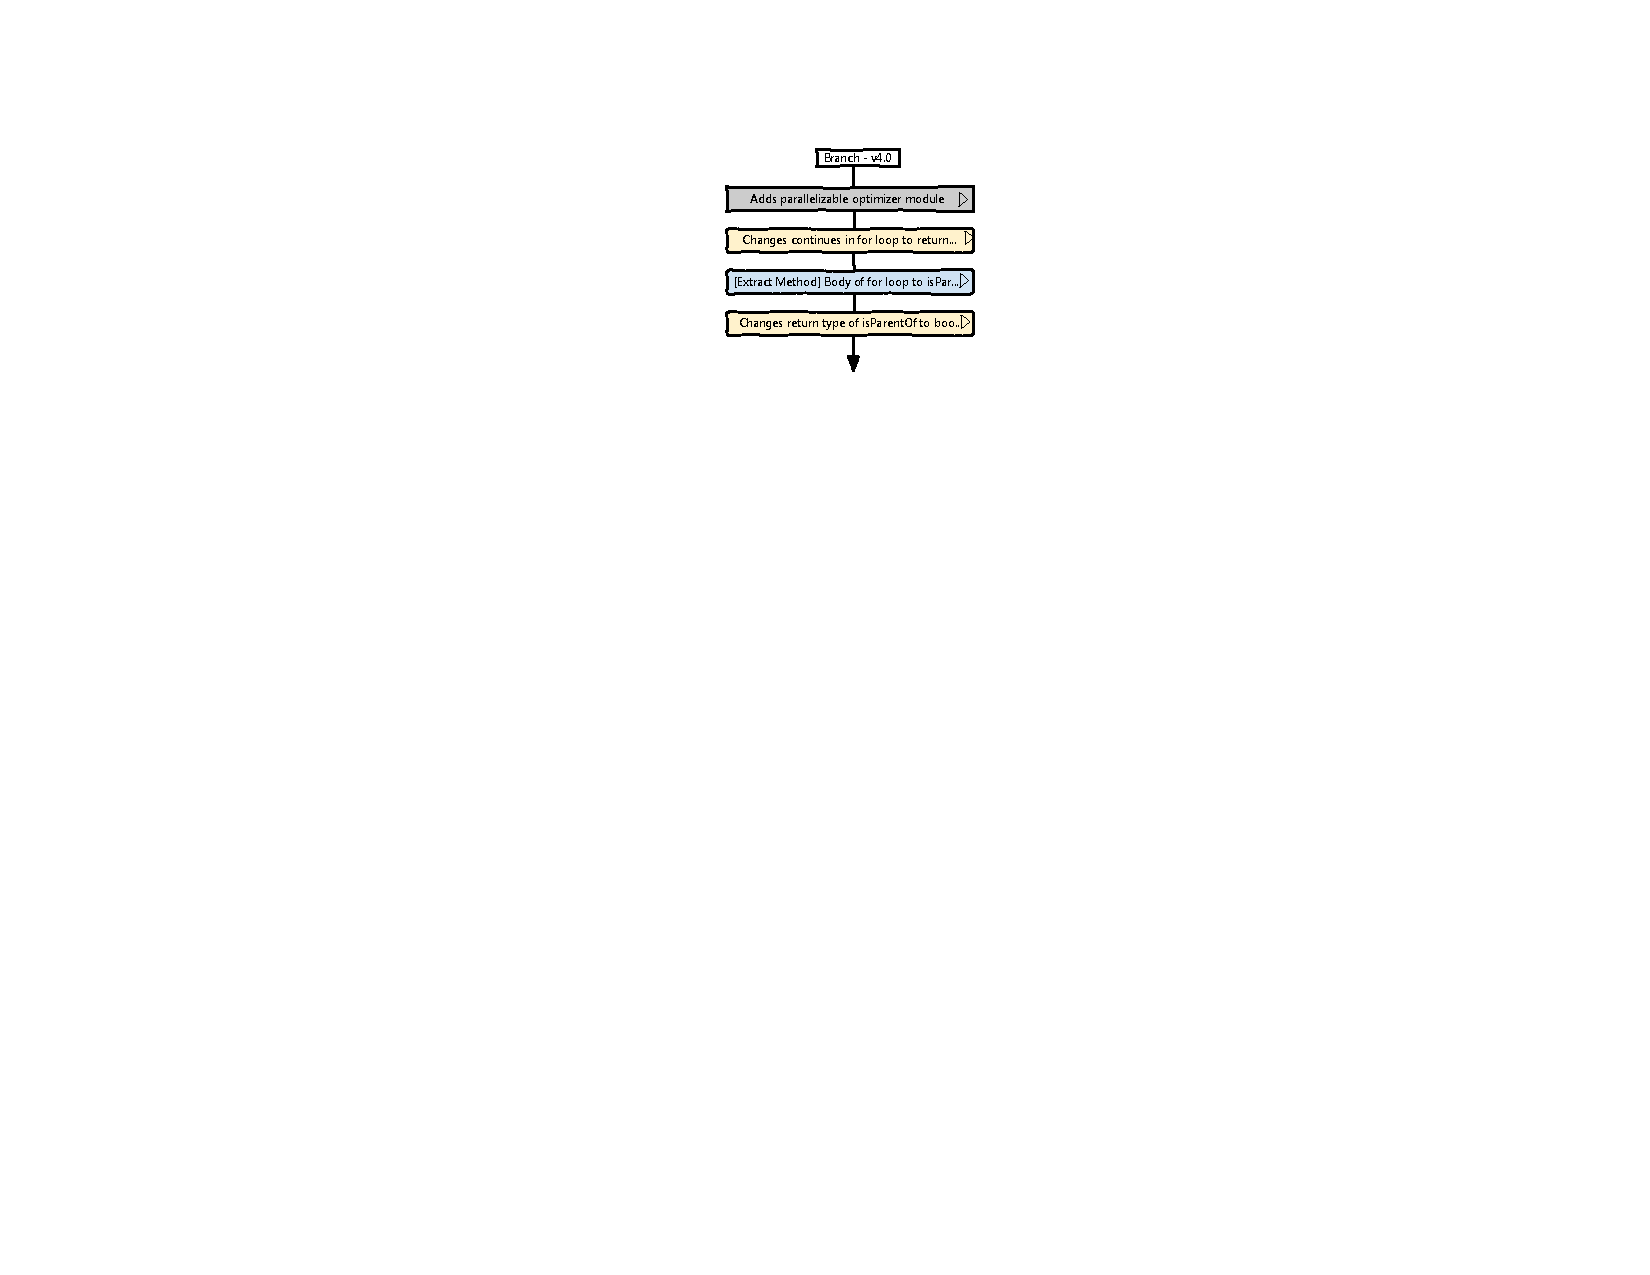
\includegraphics[height=1.9in]{presquash-history}
\caption{Commit bubbles are generated automatically while developing code. 
A solid outline indicates the commit bubble has been stored to public history, dashed outlines indicate commits that can be reordered.
These auto-generated commit bubbles give a starting point for a systematic history.}
\label{fig:presquash-history}
\end{figure}

\begin{figure}[h]
\centering
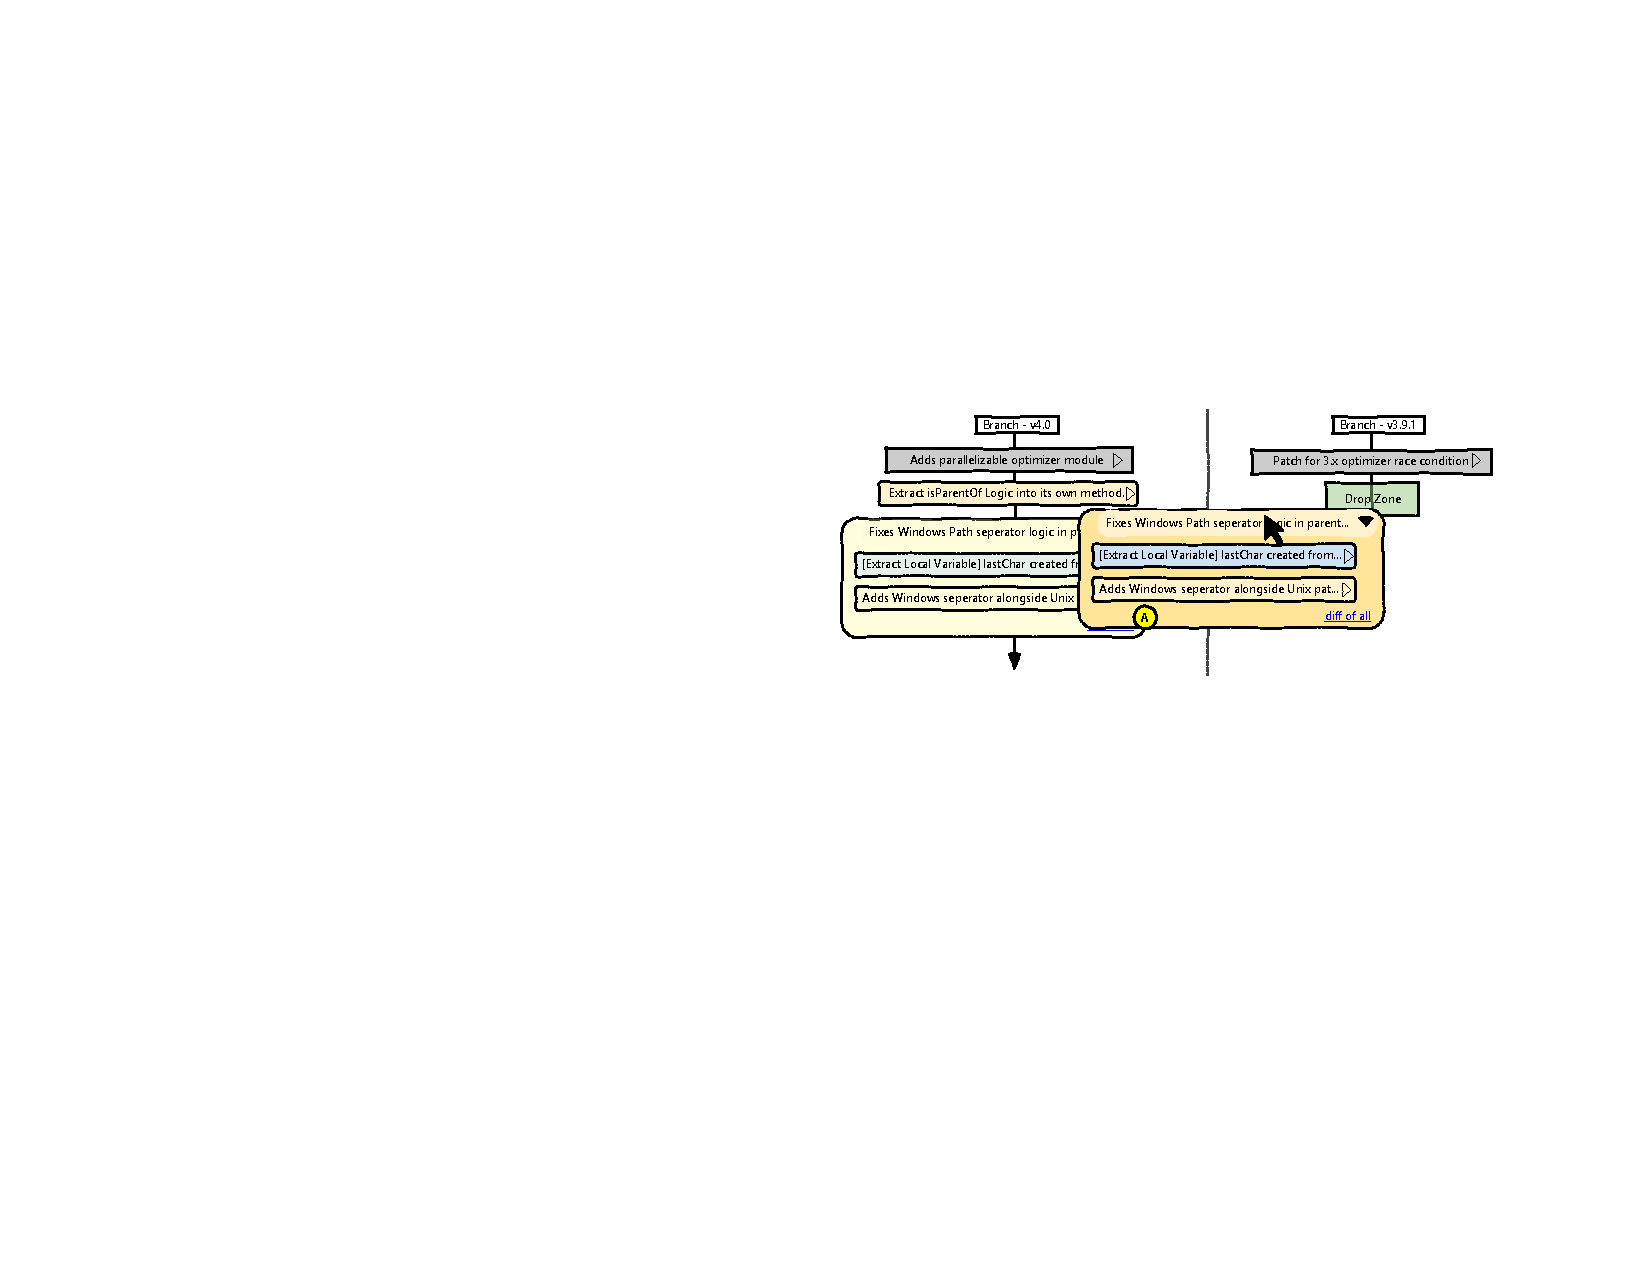
\includegraphics[width=3.0in]{cross-branch2}
\caption{Commit bubbles are copied from one branch and integrated into another by drag-and-dropping the commit bubble from the source branch to the target branch.
While existing tools optimize for making commits, our tool makes revising history tasks just as easy.
}
\label{fig:cross-branch}
\end{figure}
In existing version control tools, Anthony would not be able to easily transfer his commits across the two branches;
line-based patches do not understand the semantics of the code and fails to apply the patch.
He would not be able to transfer the refactoring commits (Figure \ref{fig:eclipse}C) and the bugfix either because the branch is in a strict ``bugfixes only'' cycle which does not allow non-essential changes such as refactorings.
Decoupling this relatively simply refactoring change from the bugfix is unexpectedly nontrivial.
One recommended ``low-tech'' way to do this would be ``save your all your edits, then re-introduce them in logical chunks, committing as you go''~\cite{GitBestPractices}.
More sophisticated approaches exist, but they are even more burdensome and error-prone because they rely on complex and non-obvious data structure-level manipulations~\cite{SausageMaking}.
Worst of all, in either approach, he would have to abandon his current working set to perform the transformation because existing tools only allow one working set at a time.

This interruption would have several consequences.
Anthony might forget details of his original task, for example, that \texttt{shouldIgnoreOptionalProblems} is in a broken state.
Even if he does remember, he is now forced to recreate his working set, which duplicates work he had already done~\cite{Ko2006}.

\begin{figure}
\centering
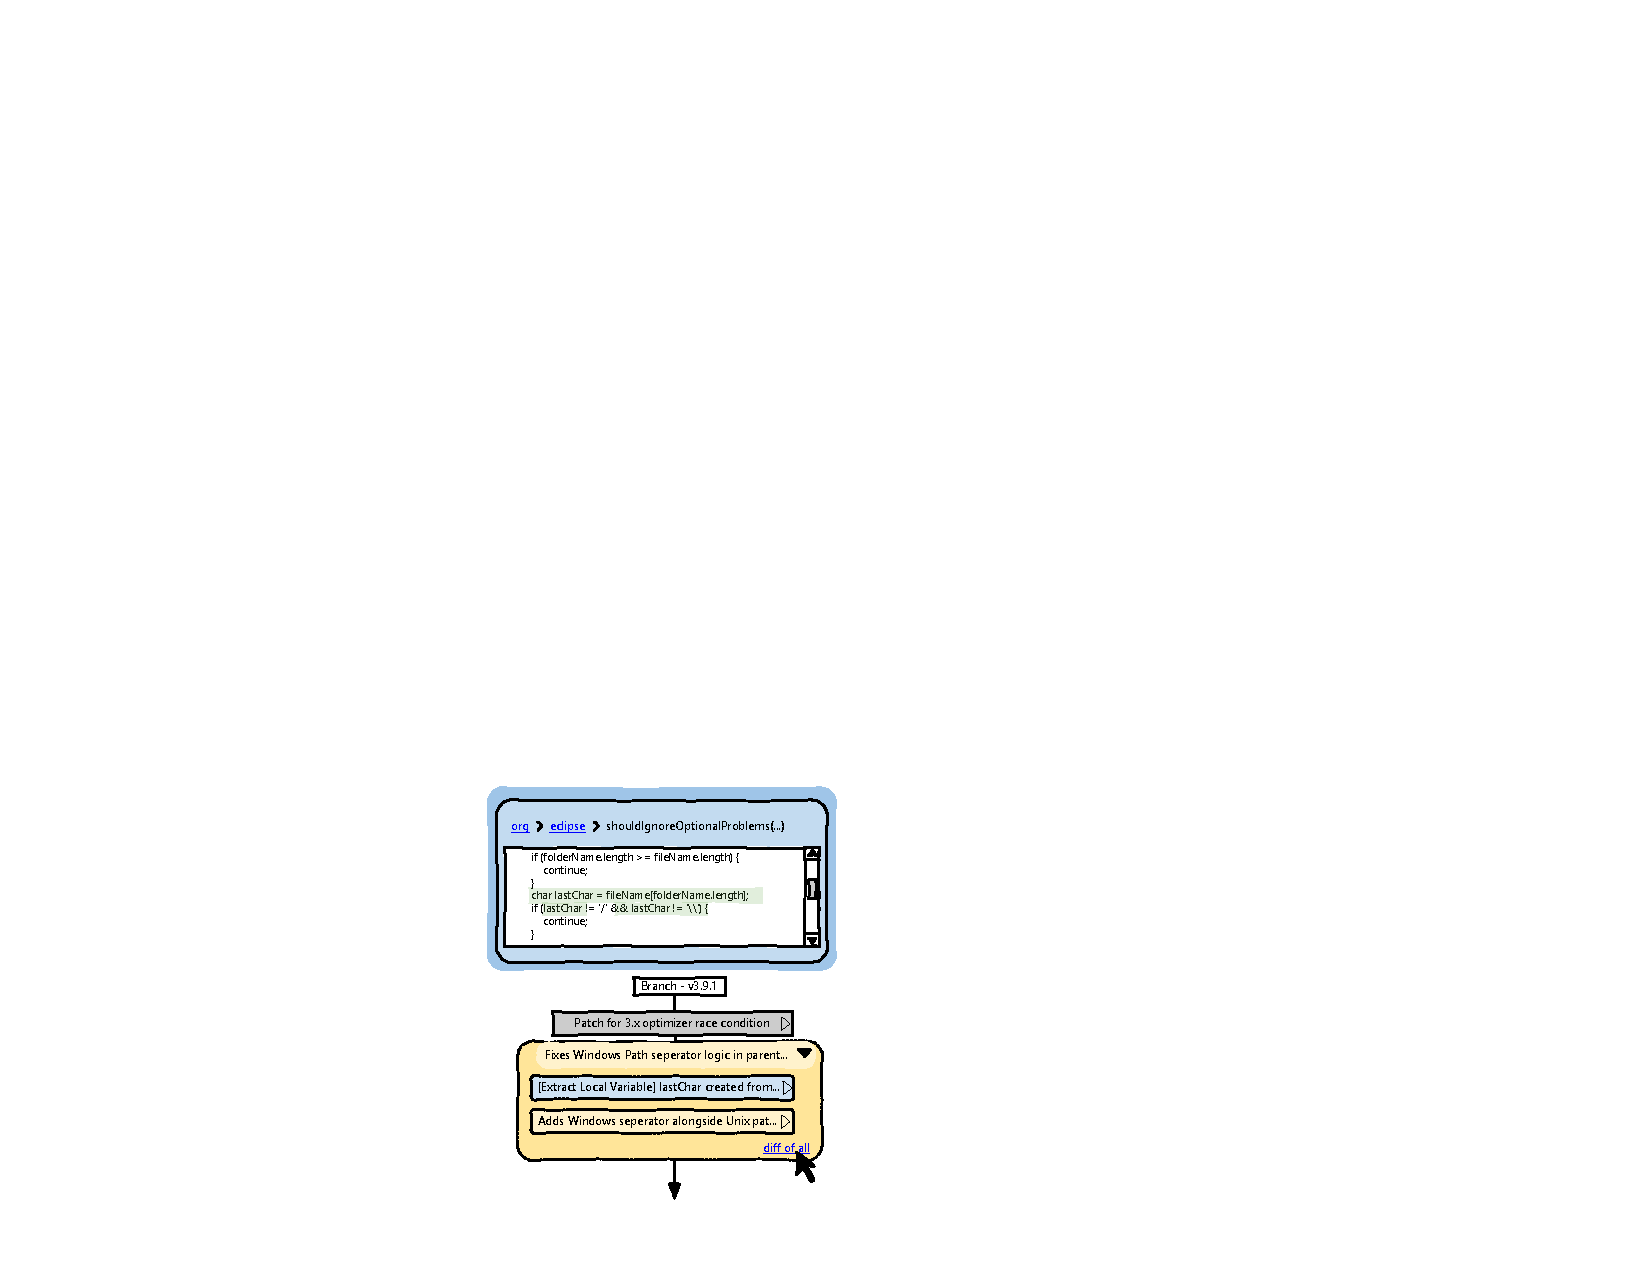
\includegraphics[width=2.2in]{cross-branch-diff}
\caption{An inline diff visualization of a squashed commit bubble. The diff is presented on an already-visible code bubble present within in the current task context to minimize context switching.}
\label{fig:diff}
\end{figure}

With Commit Bubbles, Anthony obtains the same result without breaking his flow; after writing the bugfix, he simply drags his two commits to the 3.9.1 working set and verifies the diff looks correct (Figures \ref{fig:cross-branch} and \ref{fig:diff}, respectively).
Commit Bubbles keeps track of the different contexts and utilizes AST- and heuristic-based algorithms (see Section \ref{sec:challenges}), to fluidly perform these history changes.
Incidentally, since Anthony did not have to context switch, he quickly resumes properly handling the return value of \texttt{isParentOf}.

\section{Emerging Results}

We have conducted an informal pilot study ($n = 5$) in which participants from our lab were asked to perform an activity similar to the one described in Section~\ref{sec:userexperience} using Git\footnote{\url{http://www.git-scm.com/}}.
We found that even though participants could verbally describe the history revision they needed, they were unable to actually accomplish the task. The participants had to frequently switch between different tools, and the revision commands needed to perform the action were unintuitive (e.g., \emph{rebase}).

Moreover, we found that participants verbally described operations in terms of code fragments, e.g., ``move this conditional statement,'' yet version control tools required them to think in terms of lines. 
In contrast, when developers were first given the desired commit history (e.g. systematic strategy) and then instructed to make the necessary code changes, they were able to both write the code and create the history. 
We used this preliminary feedback as an inspiration for our vision.

\section{Challenges}
\label{sec:challenges}
We articulate technical and usability challenges that we face in realizing our vision, and while doing so, reference related work that makes progress towards these areas.  

\textbf{Technical challenges.} Two technical challenges of note require techniques that can automatically generate commits in real time and more robustly rearange commit history.
Generating commits is straight forward when the developer explicitly uses a tool, but research has shown that many developers perform operations manually, even when an automatic tool is available~\cite{Murphy-Hill2012c}.
Towards these efforts, Negara and colleagues have proposed AST-based (rather than text-based) approaches to capturing edit sequences at an appropriate level of abstraction~\cite{Negara2012}. Similarly, Kirinuki and colleagues uses past commits to determine if a proposed commit may include a tangled change~\cite{Kirinuki2014}. 
Buse and colleagues offer an automatic technique for synthesizing human-readable documentation for arbitrary program differences~\cite{Buse2010}.
Finally, we are particularly encouraged by the impressive work of Hayashi and colleagues, who have proposed an algorithm for refactoring commit histories without impacting the resulting code~\cite{Hayashi2012}. 
We think the advancement of these technical obstacles are critical to implementing our vision.

\textbf{Usability challenges.} We posit that blending coding activities with commit activities solves several key obstacles to generating best-practice commit histories, but the blending process introduces its own challenges. 
First, it is possible that keeping coding and commit activities as separate activities has its own cognitive benefits, and that these benefits are lost when these activities are unified. 
It is also possible that developers do not find the unification of these activities supports their flow; instead, they may be perceived as interruptions~\cite{Parnin2012}. 
In addition, we have not yet addressed the problem of ``bubble'' overload, in which multiple bubbles for different tasks present themselves to the developer simultaneously, resulting in task contexts unmanageable for the developer.
A possible avenue for addressing these issues may be recommendation systems, which appropriately reveal and dismiss information or tools as needed to support a particular task~\cite{Robillard2010a, Murphy2005}.
Further user studies are needed to validate the extent to which our approach
can generalize across other software development activities.


\section{Conclusion}

A significant barrier to creating systematic commit histories is that developers do not always work systematically; instead, they frequently work in an as-needed way. 
Our emerging results revealed that translating as-needed activities to systematic commit histories as a separate maintenance activity is a time-consuming and difficult process for developers to perform successfully. 
We proposed an alternative interaction model in which expensive cognitive context switches are minimized, and one in which exceptional situations
%, which arise frequently when developers use an as-needed strategy, 
are treated a routine part of the developer's workflow. 
Finally, we demonstrated the promise of this approach by applying these principles to version control commits using Commit Bubbles. 
Our work demonstrates the potential of tools that adapt to developers' familiar workflow, rather than constraining developers to a tool's computational model.

% \begin{figure}[!t]
% \centering
% 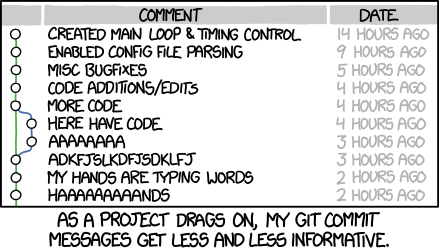
\includegraphics[width=\linewidth]{xkcd}
% \caption{This is part of the problem.}
% \label{fig:xkcd}
% \end{figure}

% An example of a floating table. Note that, for IEEE style tables, the
% \caption command should come BEFORE the table. Table text will default to
% \footnotesize as IEEE normally uses this smaller font for tables.
% The \label must come after \caption as always.
%
%\begin{table}[!t]
%% increase table row spacing, adjust to taste
%\renewcommand{\arraystretch}{1.3}
% if using array.sty, it might be a good idea to tweak the value of
% \extrarowheight as needed to properly center the text within the cells
%\caption{An Example of a Table}
%\label{table_example}
%\centering
%% Some packages, such as MDW tools, offer better commands for making tables
%% than the plain LaTeX2e tabular which is used here.
%\begin{tabular}{|c||c|}
%\hline
%One & Two\\
%\hline
%Three & Four\\
%\hline
%\end{tabular}
%\end{table}


% Note that IEEE does not put floats in the very first column - or typically
% anywhere on the first page for that matter. Also, in-text middle ("here")
% positioning is not used. Most IEEE journals/conferences use top floats
% exclusively. Note that, LaTeX2e, unlike IEEE journals/conferences, places
% footnotes above bottom floats. This can be corrected via the \fnbelowfloat
% command of the stfloats package.

% use section* for acknowledgement

\section*{Acknowledgments}

This material is based upon work supported by the National Science Foundation under Grant No. 1217700. 
We thank the Software Engineering group at ABB Corporate Research for their funding and support.
We also thank Steven P. Reiss at Brown University for introducing us to Code Bubbles.

% I did this all by myself.


% trigger a \newpage just before the given reference
% number - used to balance the columns on the last page
% adjust value as needed - may need to be readjusted if
% the document is modified later
%\IEEEtriggeratref{8}
% The "triggered" command can be changed if desired:
%\IEEEtriggercmd{\enlargethispage{-5in}}

% references section

% can use a bibliography generated by BibTeX as a .bbl file
% BibTeX documentation can be easily obtained at:
% http://www.ctan.org/tex-archive/biblio/bibtex/contrib/doc/
% The IEEEtran BibTeX style support page is at:
% http://www.michaelshell.org/tex/ieeetran/bibtex/
\bibliographystyle{IEEEtran}
% argument is your BibTeX string definitions and bibliography database(s)
\bibliography{library}



% that's all folks
\end{document}


